\section*{Exercise 1}

\subsection*{Sentence A}

\begin{center}
\begin{tabular}{| c | c |}
\hline
$Smoke$ & $Smoke \implies Smoke$ \\
\hline
$true$ & $true$ \\
\hline
$false$ & $true$ \\
\hline
\end{tabular}
\end{center}

The sentence is \textit{valid} (reflexive property, see truth table).

\subsection*{Sentence B}

\begin{center}
\begin{tabular}{| c | c | c |}
\hline
$Smoke$ & $Fire$ & $Smoke \implies Fire$ \\
\hline
$true$ & $true$ & $true$ \\
\hline
$false$ & $true$ & $true$ \\
\hline
$false$ & $false$ & $true$ \\
\hline
$true$ & $false$ & $false$ \\
\hline
\end{tabular}
\end{center}

The sentence is \textit{satisfiable} (see truth table).

\subsection*{Sentence C}

Let $B \equiv (Smoke \implies Fire)$ and $C \equiv (\neg Smoke \implies \neg Fire)$.

\begin{center}
\begin{tabular}{| c | c | c | c | c |}
\hline
$Smoke$ & $Fire$ & $B$ & $C$ & $B \implies C$  \\
\hline
$true$ & $true$ & $true$ & $true$ & $true$ \\
\hline
$false$ & $true$ & $true$ & $false$ & $false$ \\
\hline
$false$ & $false$ & $true$ & $true$ & $true$ \\
\hline
$true$ & $false$ & $false$ & $true$ & $true$ \\
\hline
\end{tabular}
\end{center}

The sentence is \textit{satisfiable} (see truth table).

\subsection*{Sentence D}

$Fire \lor \neg Fire \equiv true$ (law of excluded middle), therefore the sentence is \textit{valid}:
\smallskip
\begin{gather*}
Smoke \lor Fire \lor \neg Fire \equiv \\
Smoke \lor true \equiv \\
true
\end{gather*}

\subsection*{Sentence E}

\begin{gather*}
((Smoke \land Heat) \implies Fire) \iff ((Smoke \implies Fire) \lor (Heat \implies Fire)) \equiv \\
(\neg(Smoke \land Heat) \lor Fire) \iff ((Smoke \implies Fire) \lor (Heat \implies Fire)) \equiv \\
(\neg Smoke \lor \neg Heat \lor Fire) \iff ((Smoke \implies Fire) \lor (Heat \implies Fire)) \equiv \\
(\neg Smoke \lor \neg Heat \lor Fire) \iff ((\neg Smoke \lor Fire) \lor (\neg Heat \lor Fire)) \equiv \\
(\neg Smoke \lor \neg Heat \lor Fire) \iff (\neg Smoke \lor \neg Heat \lor Fire) \equiv \\
true
\end{gather*}

Therefore the sentence is \textit{valid}.

\subsection*{Sentence F}

\begin{gather*}
(Smoke \implies Fire) \implies ((Smoke \land Heat) \implies Fire) \equiv \\
(\neg Smoke \lor Fire) \implies ((Smoke \land Heat) \implies Fire) \equiv \\
(\neg Smoke \lor Fire) \implies (\neg (Smoke \land Heat) \lor Fire) \equiv \\
\neg (\neg Smoke \lor Fire) \lor (\neg (Smoke \land Heat) \lor Fire) \equiv \\
(Smoke \land \neg Fire) \lor (\neg (Smoke \land Heat) \lor Fire) \equiv \\
(Smoke \land \neg Fire) \lor \neg Smoke \lor \neg Heat \lor Fire \equiv \\
((Smoke \lor \neg Smoke) \land (\neg Fire \lor \neg Smoke)) \lor \neg Heat \lor Fire \equiv \\
(true \land (\neg Fire \lor \neg Smoke)) \lor \neg Heat \lor Fire \equiv \\
\neg Fire \lor \neg Smoke \lor \neg Heat \lor Fire \equiv \\
(\neg Fire \lor Fire) \lor \neg Smoke \lor \neg Heat \equiv \\
true \lor \neg Smoke \lor \neg Heat \equiv \\
true
\end{gather*}

Therefore the sentence is \textit{valid}.

\subsection*{Sentence G}

\begin{gather*}
Big \lor Dumb \lor (Big \implies Dumb) \equiv \\
Big \lor Dumb \lor \neg Big \lor Dumb \equiv \\
(Big \lor \neg Big) \lor (Dumb \lor Dumb) \equiv \\
true \lor Dumb \equiv \\
true
\end{gather*}

Therefore the sentence is \textit{valid}.

\subsection*{Sentence H}

\begin{gather*}
(Big \land Dumb) \lor \neg Dumb \equiv \\
(Big \lor \neg Dumb) \land (Dumb \lor \neg Dumb) \equiv \\
\neg Dumb \lor Big \equiv \\
Dumb \implies Big
\end{gather*}

\begin{center}
\begin{tabular}{| c | c | c |}
\hline
$Dumb$ & $Big$ & $Dumb \implies Big$ \\
\hline
$true$ & $true$ & $true$ \\
\hline
$false$ & $true$ & $true$ \\
\hline
$false$ & $false$ & $true$ \\
\hline
$true$ & $false$ & $false$ \\
\hline
\end{tabular}
\end{center}

Therefore the sentence is \textit{satisfiable}.

\section*{Exercise 2}

Let $A$ be a sentence, and $W_1,...,W_n$ the worlds in which A would be false. Then the given observation is:
\smallskip
\begin{gather}
A \equiv \neg W_1 \land ... \land \neg W_n
\end{gather}

Each world $W_i$ can be described as a conjunction of sentences, namely: 
\smallskip
\begin{gather}
W_i \equiv W_{i,1} \land ... \land W_{i,m}
\end{gather}

From (1)$\land$(2):
\smallskip
\begin{gather*}
A \equiv \\ 
\neg (W_{1,1} \land ... \land W_{1,k}) \land ... \land \neg (W_{n,1} \land ... \land W_{n,l}) \equiv \\
(\neg W_{1,1} \lor ... \lor \neg W_{1,k}) \land ... \land (\neg W_{n,1} \lor ... \lor \neg W_{n,l})
\end{gather*}

which is in CNF.

\section*{Exercise 3}

The vocabulary of the first order logic expressions contains the following predicates and constants:

\begin{itemize}

\item $Student(x)$: $x$ is a student

\item $Takes(x, c, s)$: student $x$ takes course $c$ in semester $s$ (used in both present and past tense)

\item $French$, $Greek$: constants for the corresponding courses

\item $Spring2001$: constant for the corresponding semester

\item $Passes(x, c, s)$: student $x$ passes course $c$ in semester $s$

\item $Score(x, c, s)$: the score obtained by student $x$ in course $c$ in semester $s$

\item $>(a, b)$: a is greater than b

\item $Person(x)$: $x$ is a person

\item $Policy(x)$: $x$ is a policy

\item $Buys(x, p, a)$: person $x$ buys policy $p$ from agent $a$

\item $Smart(x)$: $x$ is smart

\item $Expensive(x)$: $x$ is expensive

\item $Sells(a, p, x)$: agent $a$ sells policy $p$ to person $x$

\item $Agent(x)$: $x$ is an agent

\item $Insured(x)$: $x$ is insured

\end{itemize} 

\subsection*{Sentence A}

\begin{gather*}
\exists x \ Student(x) \land Takes(x, French, Spring2001)
\end{gather*}

\subsection*{Sentence B}

\begin{gather*}
\forall x, s \ Student(x) \land Takes(x, French, s) \implies Passes(x, French, s)
\end{gather*}

\subsection*{Sentence C}

\begin{gather*}
\exists x \forall y \ Student(x) \land Takes(x, Greek, Spring2001) \land \neg (y=x) \implies \neg Takes(y, Greek, Spring2001)
\end{gather*}

\subsection*{Sentence D}

\begin{gather*}
\exists x \ \forall y, s \ >(Score(x, Greek, s), Score(y, French, s)) 
\end{gather*}

\subsection*{Sentence E}

\begin{gather*}
\forall x \ Person(x) \land (\exists p, a \ Policy(p) \land Buys(x, p, a)) \implies Smart(x)
\end{gather*}

\subsection*{Sentence F}

\begin{gather*}
\forall x, p, a \ Person(x) \land Expensive(p) \land Policy(p) \implies \neg Buys(x, p, a)
\end{gather*}

\subsection*{Sentence G}

\begin{gather*}
\exists a \ \forall p, x \ Agent(a) \land Policy(p) \land Sells(a, p, x) \implies (Person(x) \land \neg Insured(x))
\end{gather*}

%\section*{Exercise 1}
%\label{sec:exercise1}
%
%\subsection*{Part A}
%
%Using the minimax algorithm, we assume that both players play optimally (namely the MAX player maximizes his utility value, while the MIN player minimizes the same value). Furthermore, the algorithm performs a complete depth-first exploration of the corresponding game tree (Figure \ref{fig:exercise1}), assigning the minimum or maximum utility value out of all its children nodes as a minimax value to every MIN or MAX node respectively. 
%
%In this case, MIN nodes B, C, D and E would be given the values -12, -7, -9, 2 respectively, while the starting MAX node will take the maximum of these four values, namely 2. Therefore, the resulting optimal move for the MAX player would lead to E, and the optimal response by the MIN player would then lead to the terminal node with utility value 2.
%
%\subsection*{Part B}
%
%Figure \ref{fig:exercise1} depicts the game tree.
%
%\begin{figure}[htpb]
\centering
\makebox[\textwidth]{%
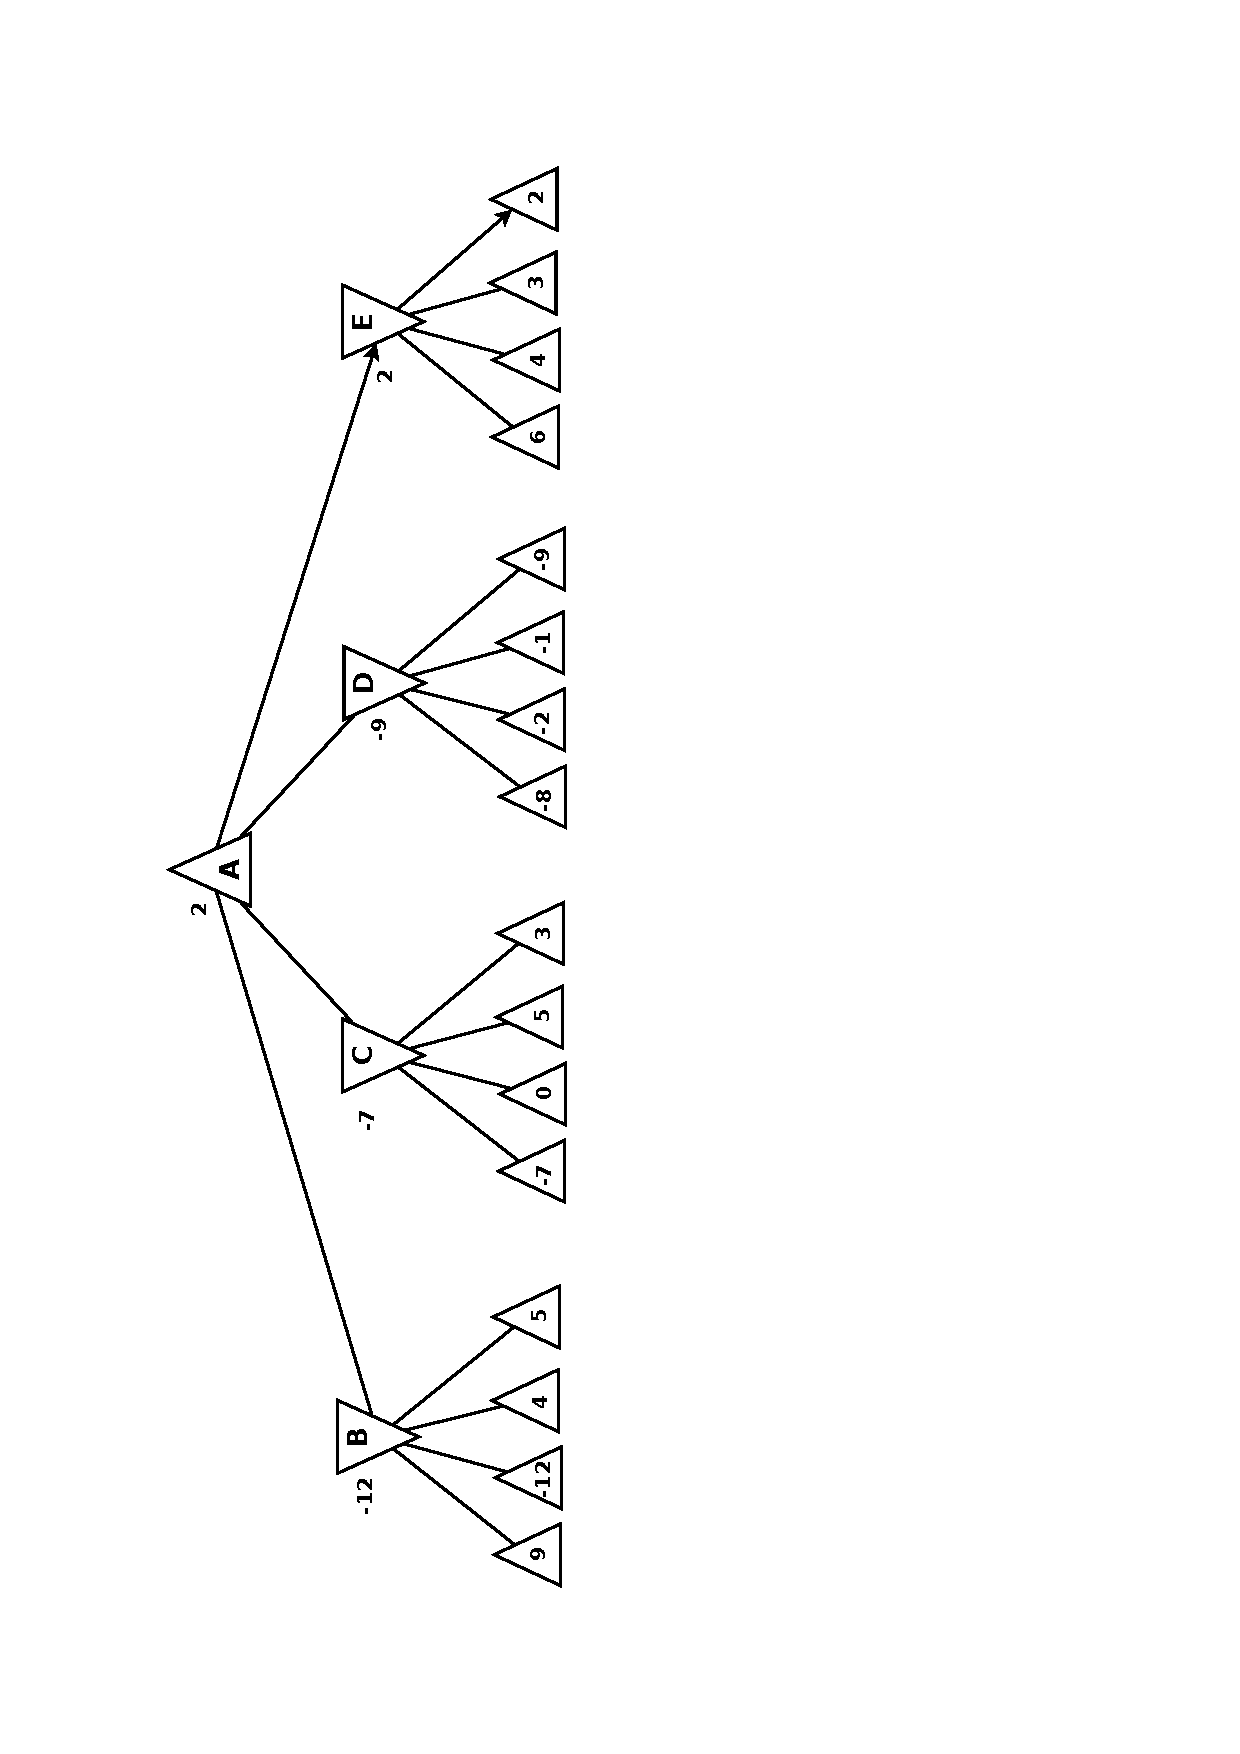
\includegraphics[width=0.3\textwidth, angle = -90, trim = 25mm 25mm 110mm 25mm,clip=true]{images/exercise1.pdf}}
\caption{The complete game tree of exercise 1. The $\bigtriangleup$ nodes represent MAX ones, whereas the $\bigtriangledown$ nodes represent MIN ones. The terminal nodes (leaves) show the utility values for MAX, whilst the other nodes are labeled with their minimax values.}
\label{fig:exercise1}
% Place the label just after the caption to make the link work
\end{figure} % table makes a floating object with a title
%
%\section*{Exercise 2}
%
%Given a binary mask $M$ and two parental solutions $A$ and $B$, their offspring $C$ produced by the genetic algorithm will inherit the value $A_i$ for each $M_i = 0$ and $B_j$ for each $M_j = 1$, where $i,j$ are indices of $A, B, M, C$. Therefore, for $A=00110101$ and $B=11010100$ the offsprings would be:
%
%a) $ M=00000111 \Rightarrow C =  00110100$
%
%b) $ M=00111000 \Rightarrow C = 00010101$
%
%c) $ M=00110110 \Rightarrow C = 00010101$
%
%\section*{Exercise 3}
%
%\subsection*{Part A}
%
%First, we need to consider that Part B requires a binary constraint satisfaction problem (CSP) because the AC-3 algorithm can only be used with binary constraints. Let $f(T_i)$ be the number of offices of department $T_i$, then the following observations lead to such a binary CSP formulation:
%
%\begin{enumerate}
%
%\item We can see from the data that $\sum_{i=1}^{12} f(T_i)=120$, in other words the company needs 120 offices in total. Given that each floor can provide at most 40 offices, each floor must have all its offices occupied (otherwise the sum of occupied offices will not be 120 and consequently not all departments will be housed).
%
%\item Since each floor will have exactly 40 occupied offices, we can easily find the lower and upper bound for the number of departments per floor. By summing the offices of the three largest departments ($f(T_3)+f(T_4)+f(T_6)=36$), we deduce that each floor must have $\ge$4 departments. Moreover, if a floor houses $>$4 departments, then at least one floor must have $<$4 departments, which is a contradiction. Therefore, each floor will house exactly 4 departments.
%
%\item We know that some departments should be on the same floor ($T_1$ with $T_3$, $T_2$ with $T_4$, $T_8$ with $T_9$). Since no combination of these pairs can occupy exactly 40 offices ($f(T_1)+f(T_3)+f(T_2)+f(T_4) = 39$, $f(T_1)+f(T_3)+f(T_8)+f(T_9) = 38$ and $f(T_2)+f(T_4)+f(T_8)+f(T_9) = 37$), we conclude that each pair should be assigned to a different floor.
%
%\end{enumerate}
%
%We are now able to define the binary CSP problem. Let $X_i \in \{T_5, T_6, T_7, T_{10}, T_{11}, T_{12}\}$, $i \in \{1, 2, 3, 4, 5, 6\}$ be the remaining departments to be allocated, then the binary constraints will be:
%
%\[
%	\begin{array}{ll}
%		X_i \ne X_j, \forall (i,j) : i \ne j \\
%		f(X_1) + f(X_2) + f(T_1) + f(T_3) = 40 \Rightarrow f(X_1) + f(X_2) = 20 \\
%		f(X_3) + f(X_4) + f(T_2) + f(T_4) = 40 \Rightarrow f(X_3) + f(X_4) = 21 \\
%		f(X_5) + f(X_6) + f(T_8) + f(T_9) = 40 \Rightarrow f(X_5) + f(X_6) = 22
%	\end{array}
%\]
%
%\subsection*{Part B}
%
%\begin{table}[htpb]
\centering
\makebox{
\resizebox{!}{1.95cm}{
\begin{tabular}{| c | c | p{3.7cm} | p{3.7cm} | p{3.7cm} |}
\hline
& Initial Domain & $(X_1 \ne X_2) \cap (f(X_1) + f(X_2) = 20)$ & $(X_3 \ne X_4) \cap (f(X_3) + f(X_4) = 21)$ & $(X_5 \ne X_6) \cap (f(X_5) + f(X_6) = 22)$\\
\hline
$X_1$ & $T_5, T_6, T_7, T_{10}, T_{11}, T_{12}$ & $T_5, T_7, T_{10}, T_{11}, T_{12}$ & $T_5, T_7, T_{10}, T_{11}, T_{12}$ & $T_5, T_7, T_{10}, T_{11}, T_{12}$ \\
\hline
$X_2$ & $T_5, T_6, T_7, T_{10}, T_{11}, T_{12}$ & $T_5, T_7, T_{10}, T_{11}, T_{12}$ & $T_5, T_7, T_{10}, T_{11}, T_{12}$ & $T_5, T_7, T_{10}, T_{11}, T_{12}$ \\
\hline
$X_3$ & $T_5, T_6, T_7, T_{10}, T_{11}, T_{12}$ & $T_5, T_6, T_7, T_{10}, T_{11}, T_{12}$ & $T_5, T_6, T_7, T_{10}, T_{11}, T_{12}$ & $T_5, T_6, T_7, T_{10}, T_{11}, T_{12}$ \\
\hline
$X_4$ & $T_5, T_6, T_7, T_{10}, T_{11}, T_{12}$ & $T_5, T_6, T_7, T_{10}, T_{11}, T_{12}$ & $T_5, T_6, T_7, T_{10}, T_{11}, T_{12}$ & $T_5, T_6, T_7, T_{10}, T_{11}, T_{12}$ \\
\hline
$X_5$ & $T_5, T_6, T_7, T_{10}, T_{11}, T_{12}$ & $T_5, T_6, T_7, T_{10}, T_{11}, T_{12}$ & $T_5, T_6, T_7, T_{10}, T_{11}, T_{12}$ & $T_6, T_7, T_{10}, T_{11}, T_{12}$ \\
\hline
$X_6$ & $T_5, T_6, T_7, T_{10}, T_{11}, T_{12}$ & $T_5, T_6, T_7, T_{10}, T_{11}, T_{12}$ & $T_5, T_6, T_7, T_{10}, T_{11}, T_{12}$ & $T_6, T_7, T_{10}, T_{11}, T_{12}$ \\
\hline
\end{tabular}
}}
\caption{The initial progress of the AC-3 algorithm for the first three (and their reverse) arcs. The columns contain the initial domain of each variable, and the updated domains after considering the first three (and their reverse) arcs of the queue.}
\label{table:ac3}
\end{table}
%
%The aforementioned constraint equations contain 30 arcs in total (since all nodes of its undirected graph representation are connected with each other and arcs are directed). Assume that the initial queue of arcs given to AC-3 is $[(X_1 \ne X_2) \cap (f(X_1) + f(X_2) = 20), (X_3 \ne X_4) \cap (f(X_3) + f(X_4) = 21), (X_5 \ne X_6) \cap (f(X_5) + f(X_6) = 22), X_1 \ne X_3, X_1 \ne X_4, ..., X_4 \ne X_6]$. Then the first iteration of AC-3 is to remove the first arc (and its reverse) and check each value in the domain of $X_1$ (and $X_2$ respectively) for inconsistencies. The updated domain is then $X_1, X_2 \in \{T_5, T_7, T_{10}, T_{11}, T_{12}\}$. Since the domain of $X_1$ (the same applies for $X_2$) has been updated, each arc ($X_k$,$X_1$), $k\ne1$ need to be added in the queue for rechecking (in the first iteration all these arcs are already in the queue).
%
%The following iterations continue in a similar fashion until either the queue (success) or a domain (failure) is empty. Table \ref{table:ac3} shows how the domain is updated for the first three (six if we count the reverse arcs separately) iterations of the algorithm.
%
%
%\section*{Exercise 4}
%
%As explained in Exercise 1, the minimax algorithm guarantees the optimal solution for the MAX player given that both players make optimal decisions. Assuming that the MIN player chooses a suboptimal action instead, then the value of the respective MIN node (and thus the resulting minimax value of its parental MAX node) cannot decrease because the optimal action already led to the minimum value. The same argument can inductively be expanded to the whole game tree, proving the assertion.
%
%Giving an example, in Figure \ref{fig:exercise1} let the MIN player always select the second best available action. These suboptimal moves would then mean that the MAX player would receive 4, 0, -8 or 3 if he opted for B, C, D or E respectively. Since the optimal move found by minimax leads to E, the resulting value would increase from 2 to 3. However, moving to B would actually result in an even better value (4), thus illustrating that when the MAX player can predict a suboptimal play by MIN, there may be better strategies than following the minimax decision.






